%csky stuff
\chapter{Time-Integrated Search}

\section{Analysis properties}


\subsection{Background space PDF}

\begin{figure}
    \centering
    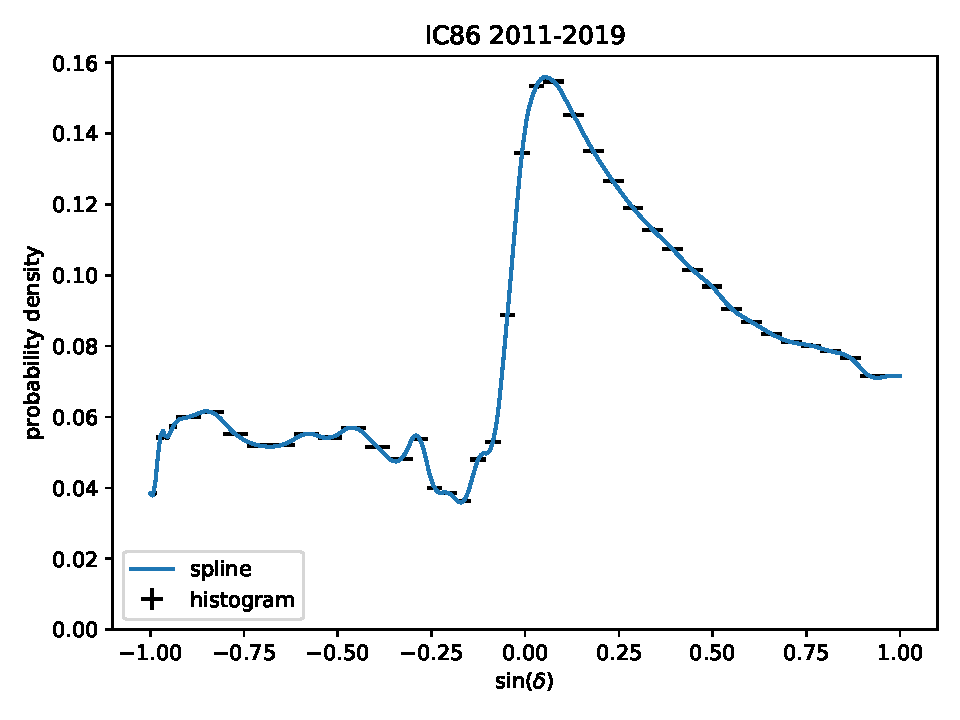
\includegraphics[width=\linewidth]{Plots/05_csky/bg_space_pdf.pdf}
    \caption{Background space PDF used in this analysis in $\sin{(\delta)}$ for all $\num{9}$ years, 2011-2019.}
\end{figure}

The background space parametrization results in one plot only because all datasets underwent the same data processing pipeline.

\subsection{Energy ratio PDF}

\begin{figure}
    \centering
    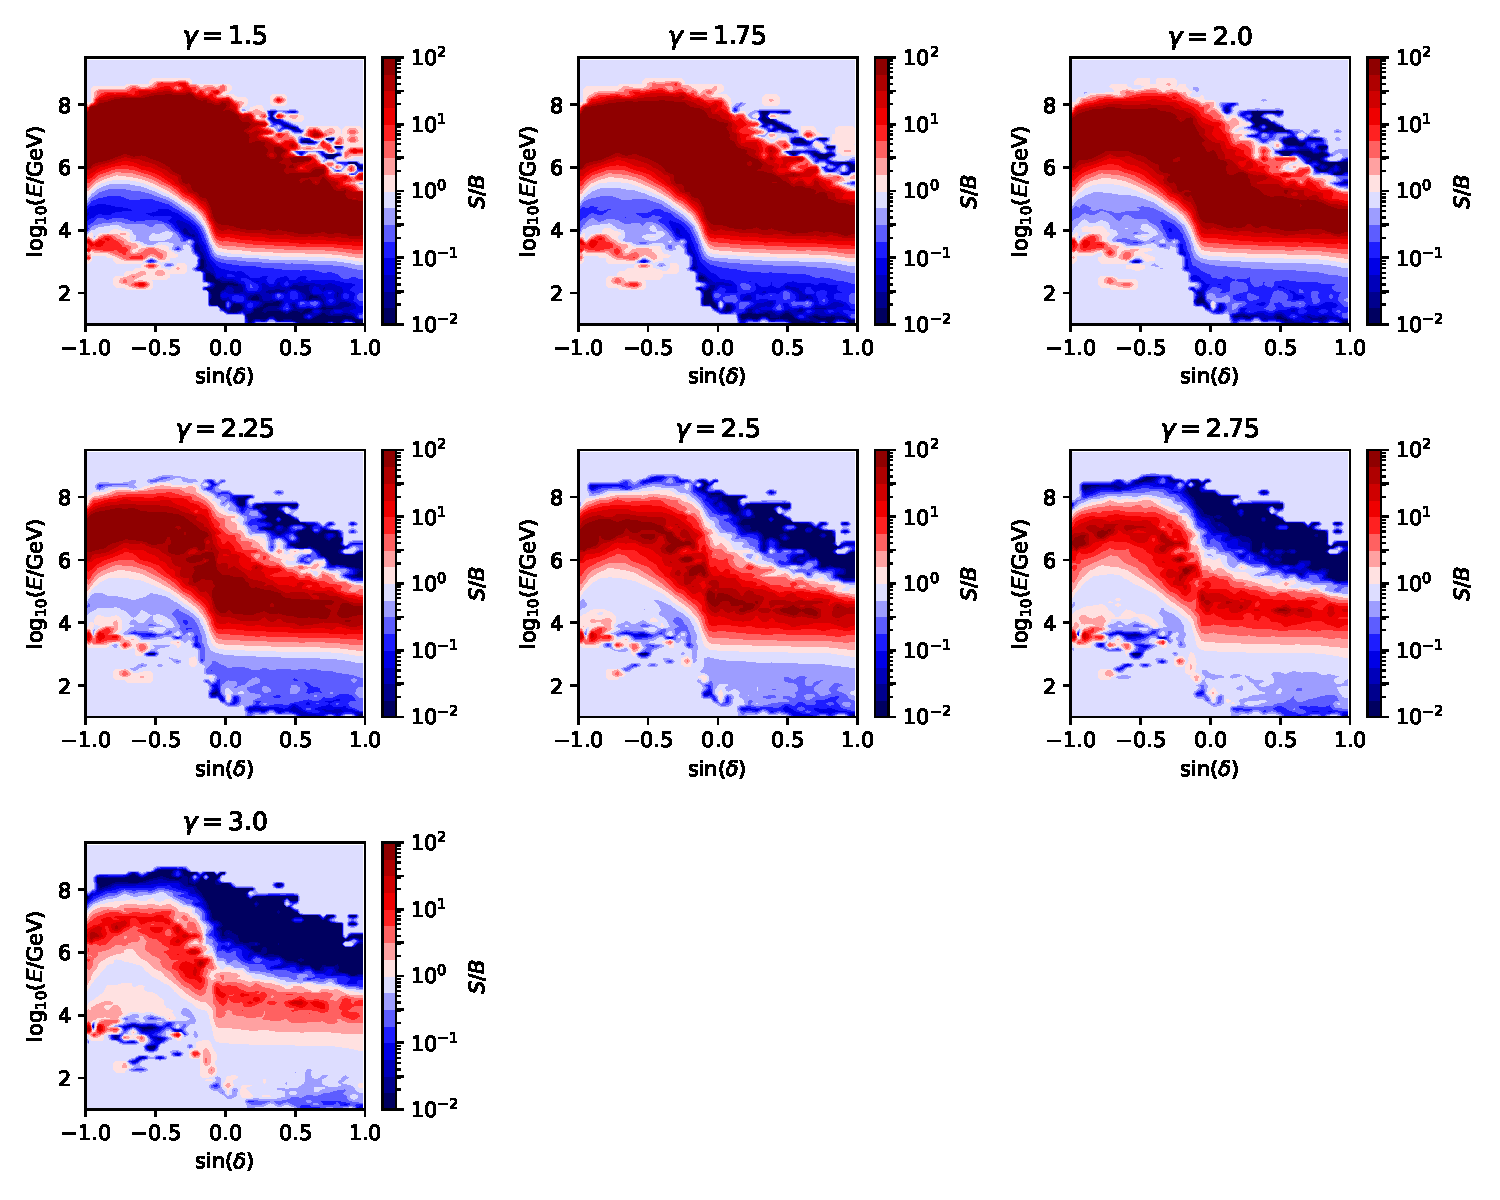
\includegraphics[width=\linewidth]{Plots/05_csky/energy_pdf_ratio.pdf}
    \caption{Energy PDF ratios used in this analysis in $\sin{(\delta)}$ and $\sin{\log{(E)}}$ for all $\num{9}$ years, 2011-2019, for different spectral indices $gamma$.}
\end{figure}

Mention high values in upper right (okay since they bias towards lower sens values (weaken)) and lower left (bad, bias towards higher sens values)

\section{Background Trials}

The histogram of the background test statistic values can be seen in figure \ref{fig:bg_ts_time_int}.
The number of trials processed is $\num{974000}$\footnote{Originally $\num{e6}$, but some jobs fail due to various technical reasons.}.
Important features of the plot are that the $\chi^2$ distribution has as straight a tail as possible.
This is reflected in the number of degrees of freedom $dof$ in the $\chi^2$ distribution.
This should be as close to 1 as possible, which corresponds to a pure background statistic without signal.
The test statistic should also be symmetrical around the zero point.
A shift around the zero point is an indication of an undesired bias of the statistic.
Therefore, the value of the quotient of the number of positive and negative events should ideally be $\eta = \num{0.5}$.
Apart from the fit parameters, the median and $5\sigma$ deviation value of the test statistic are necessary for the subsequent calculation of the sensitivity and the discovery potential.

The fit parameters of the background test statistic are
\begin{align}
  dof &= \num{1.115},\\
  \eta &= \num{0.656}
\end{align}
and the key values later to be processed are as follows\footnote{Some analyses use the $3\sigma$ value for the discovery potential}
\begin{align}
  median &= \num{0.140},\\
  3\sigma &= \num{10.651},\\
  5\sigma &= \num{28.060}.
\end{align}

\begin{figure}
    \centering
    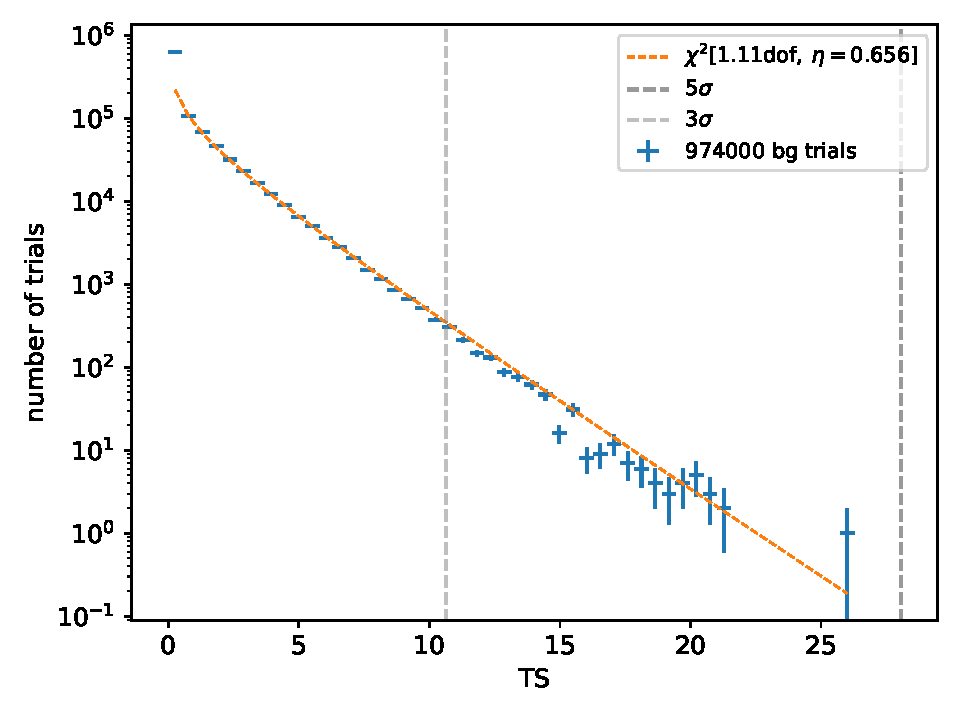
\includegraphics[width=\linewidth]{Plots/05_csky/9_years_gfu_gold_bg_new.pdf}
    \caption{Histogram of the background test statistic for the time integrated analysis. Shown are also the number of degrees of freedom $dof$ and the ratio of positive and negative values $\eta$.}
    \label{fig:bg_ts_time_int}
\end{figure}

\section{Signal Trials}

Before calculating the sensitivities and discovery potentials, certain properties of the likelihood or its behaviour should be investigated.
Since the spectral index $\gamma$ and the signal parameter $n_\text{S}$ are fitted, it is advisable to look at the likelihood environment to check the quality of the fit and exclude any other unwanted maxima.
A scan of the parameter space for one likelihood can be seen in figure \ref{fig:llh_scan_time_int}.
Although there is a relatively flat maximum, the likelihood environment does not show any strange behaviour.
\begin{figure}
    \centering
    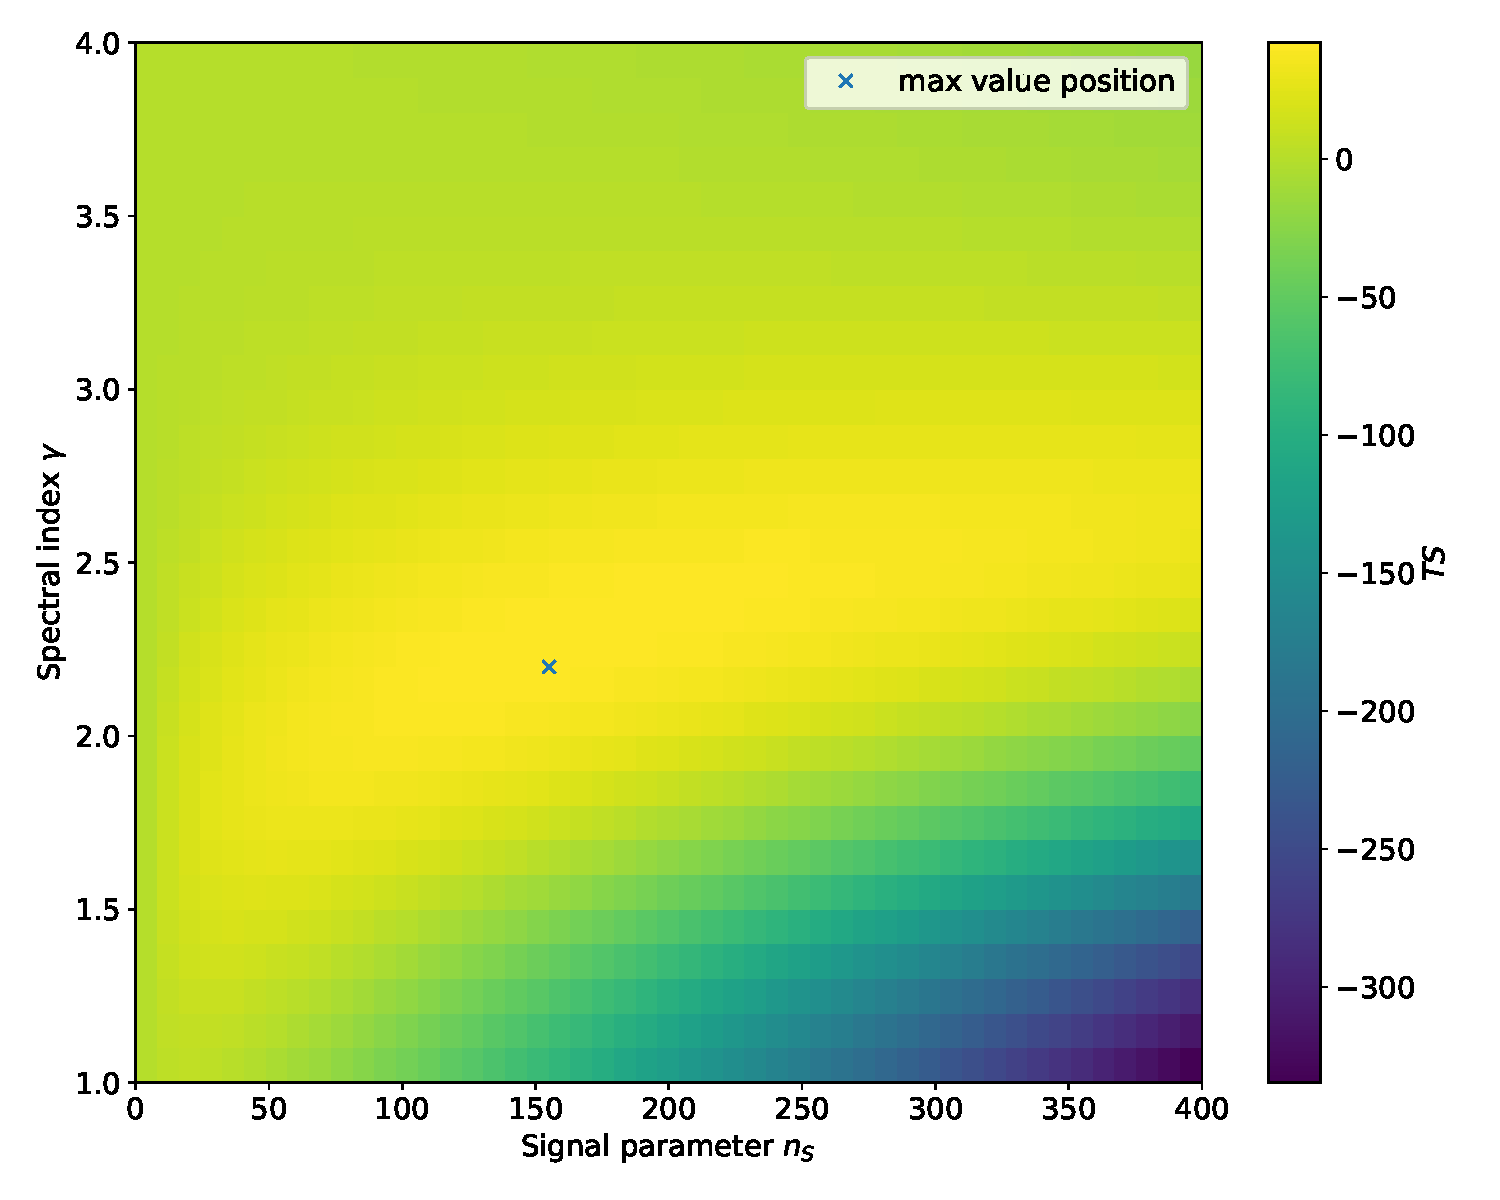
\includegraphics[width=\linewidth]{Plots/05_csky/llh_scan_time_int.pdf}
    \caption{Scan of the likelihoodspace for the time integrated analysis. The number of induced signal events is $n_S = \num{100}$ with a spectral index of $\gamma = 2$. The maximum test statistic value is marked in the plot.}
    \label{fig:llh_scan_time_int}
\end{figure}
The method of the calculation of the contours comes from \cite{Blobel} and corresponds to the maximum of the negative log-likelihood after subtracting $\num{0.5}$ and $\num{2}$ accordingly to get the $1\sigma$ and $2\sigma$ range, respectively.

After the fit behaviour has been checked, the signal can be injected.
With a higher number of signal events, the test statistic shifts to higher values, eventually reaching the thresholds set for the sensitivity and discovery potential.
Practically csky provides methods to apriori get an estimation of the number of signal events that have to be injected to satisfy certain thresholds without having to run a lot of trials on a cluster first.
The determined list of the number of signal events injected for the trials can be seen in table \ref{tab:signal_injected}.
The resulting CDFs for the time integrated sensitivities and discovery potentials can be seen in figure \ref{fig:cdf_sens} and \ref{fig:cdf_disc}.
Each point corresponds to the percentage of the test statistic being passed the thresholds mentioned in chapter \ref{sec:theory}.
\begin{figure}
    \centering
    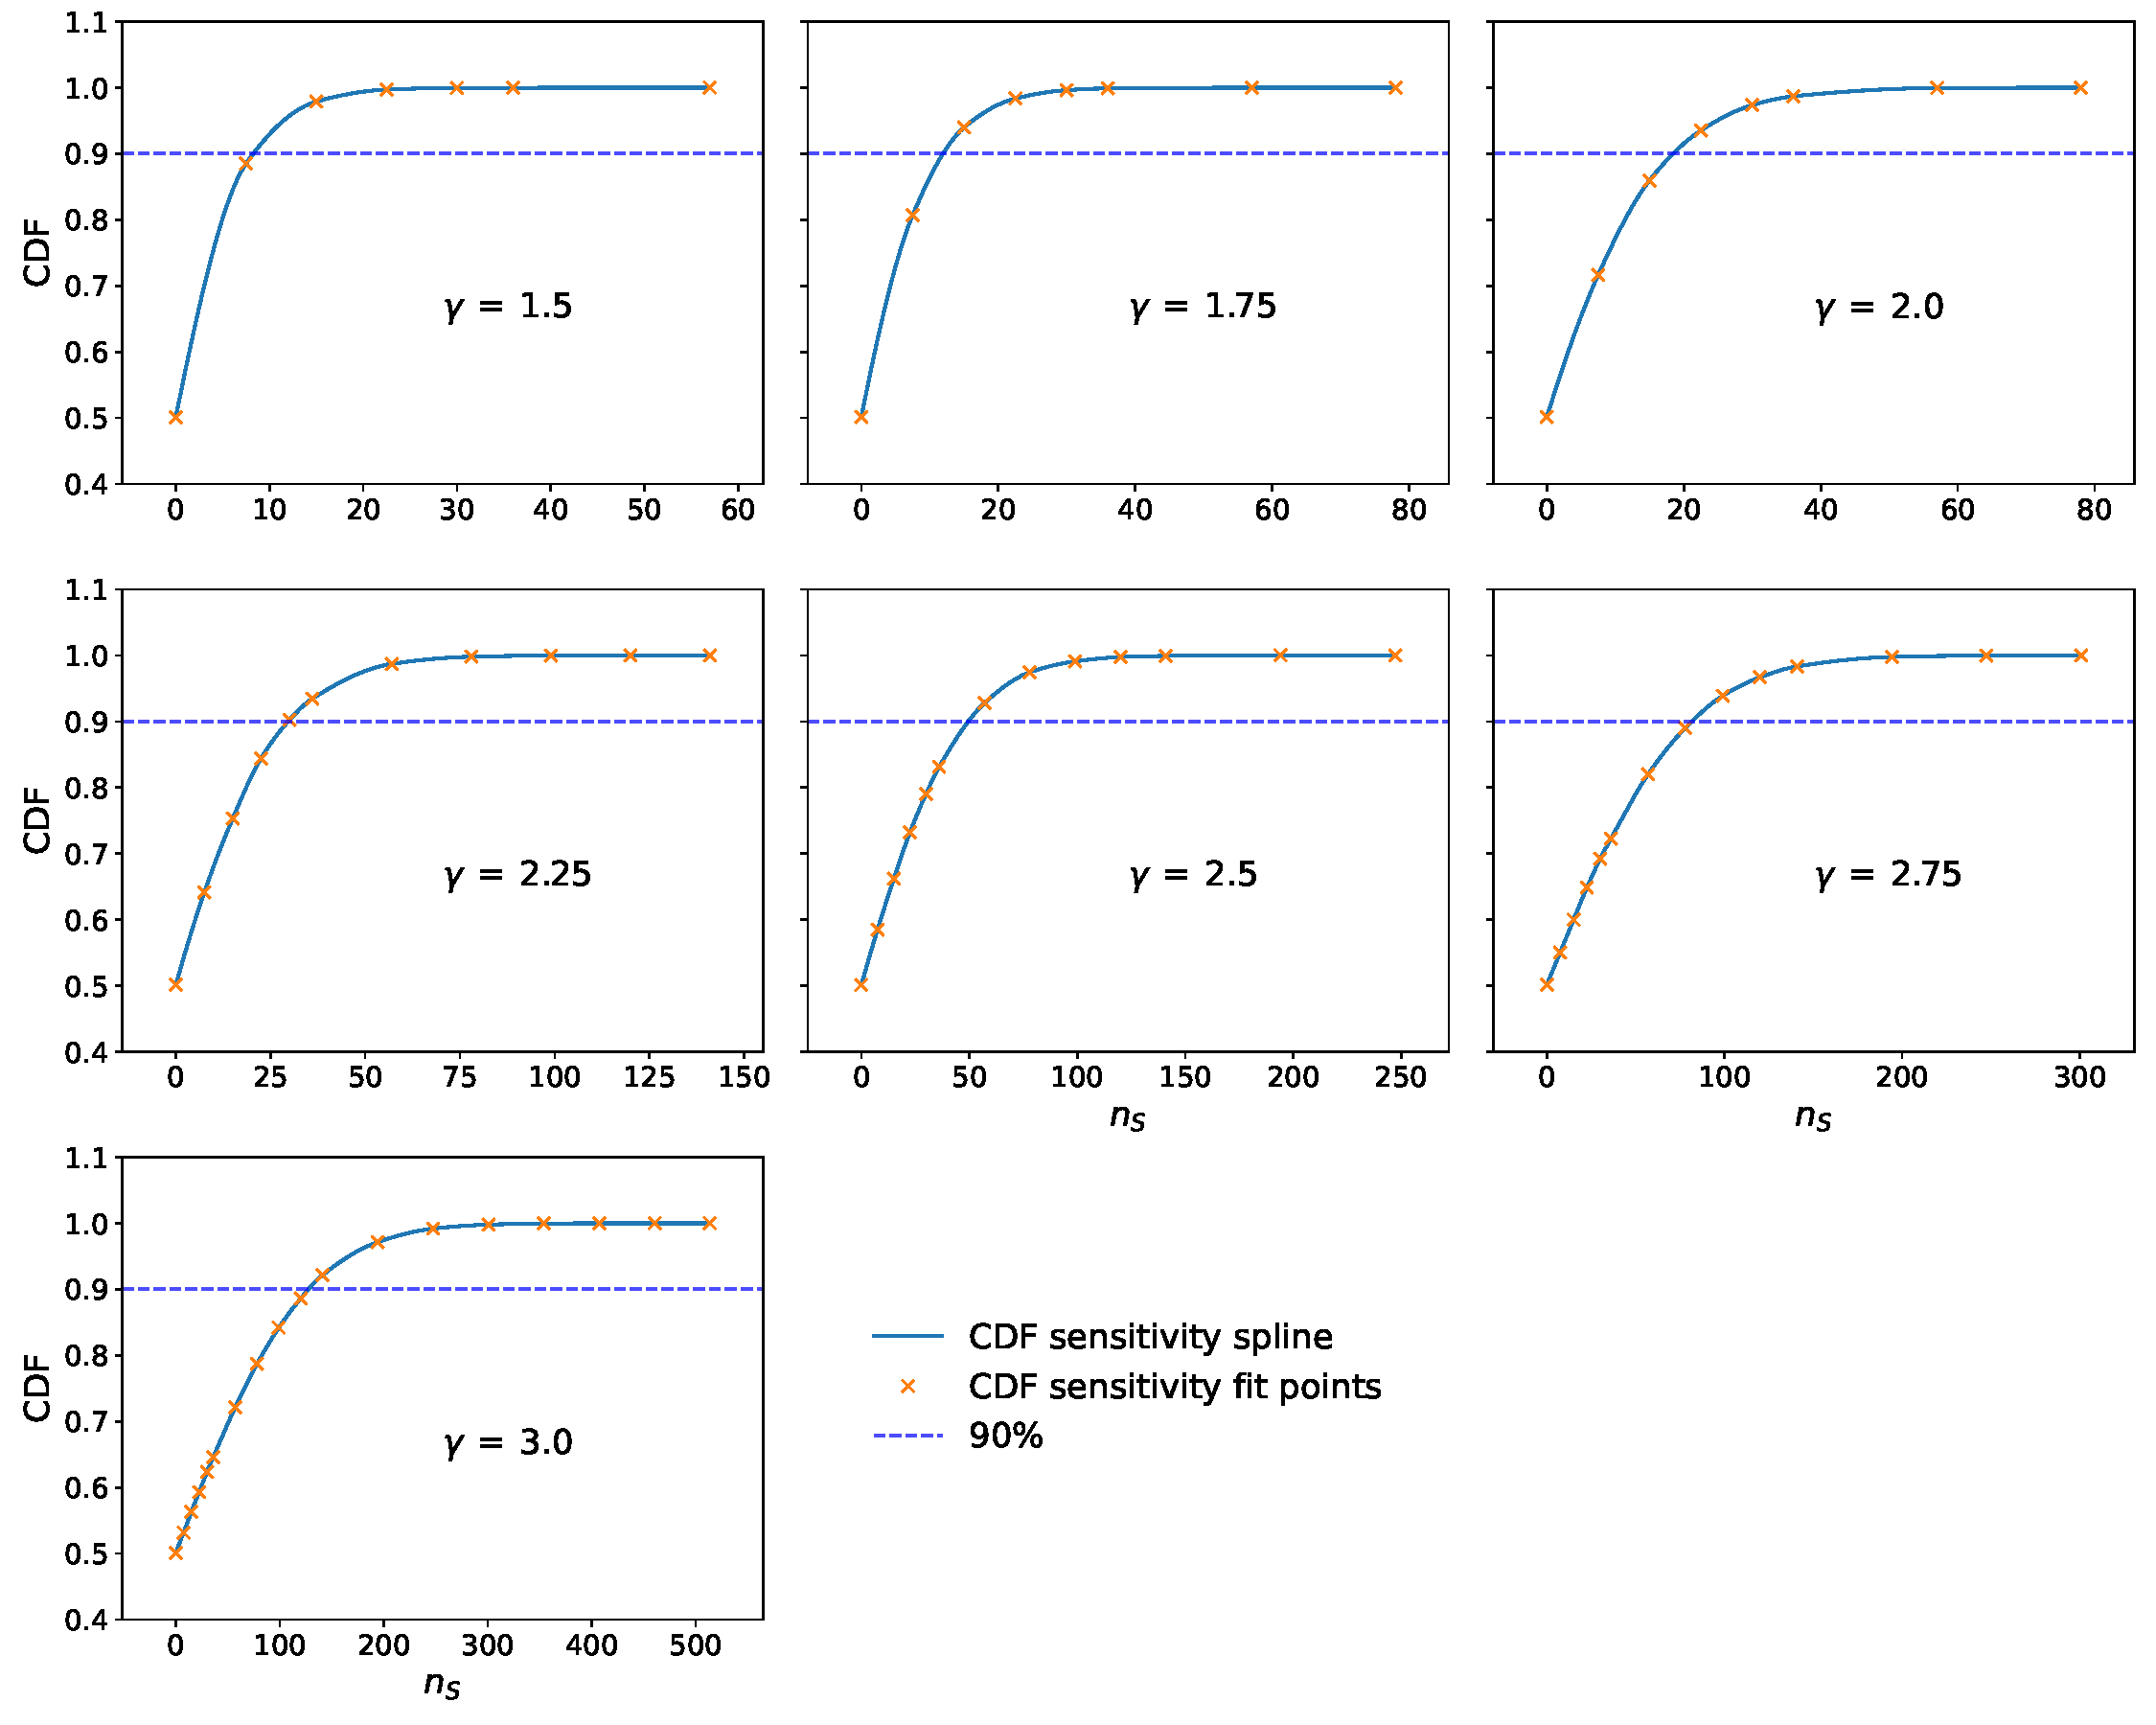
\includegraphics[width=\linewidth]{Plots/05_csky/9_years_gfu_gold_cdf_sens.pdf}
    \caption{Quantiles of the signal trials for the calculation of the sensitivity for different spectral indices $\gamma$. A $\chi^2$ CDF fit provides a more accurate estimate of the sought signal parameter $n_\text{S}$ which satisfies the sensitivity condition at $\SI{90}{\percent}$.}
    \label{fig:cdf_sens}
\end{figure}
Note that all plots in figure \ref{fig:cdf_sens} start at about $\SI{50}{\percent}$ with a signal parameter of $n_\text{S} = 0$.
Since the absence of a signal parameter produces the background test statistic, the statistics share the same median, hence there will always be $\SI{50}{\percent}$ of the signal test statistic above the median of the background test statistic.
\begin{figure}
    \centering
    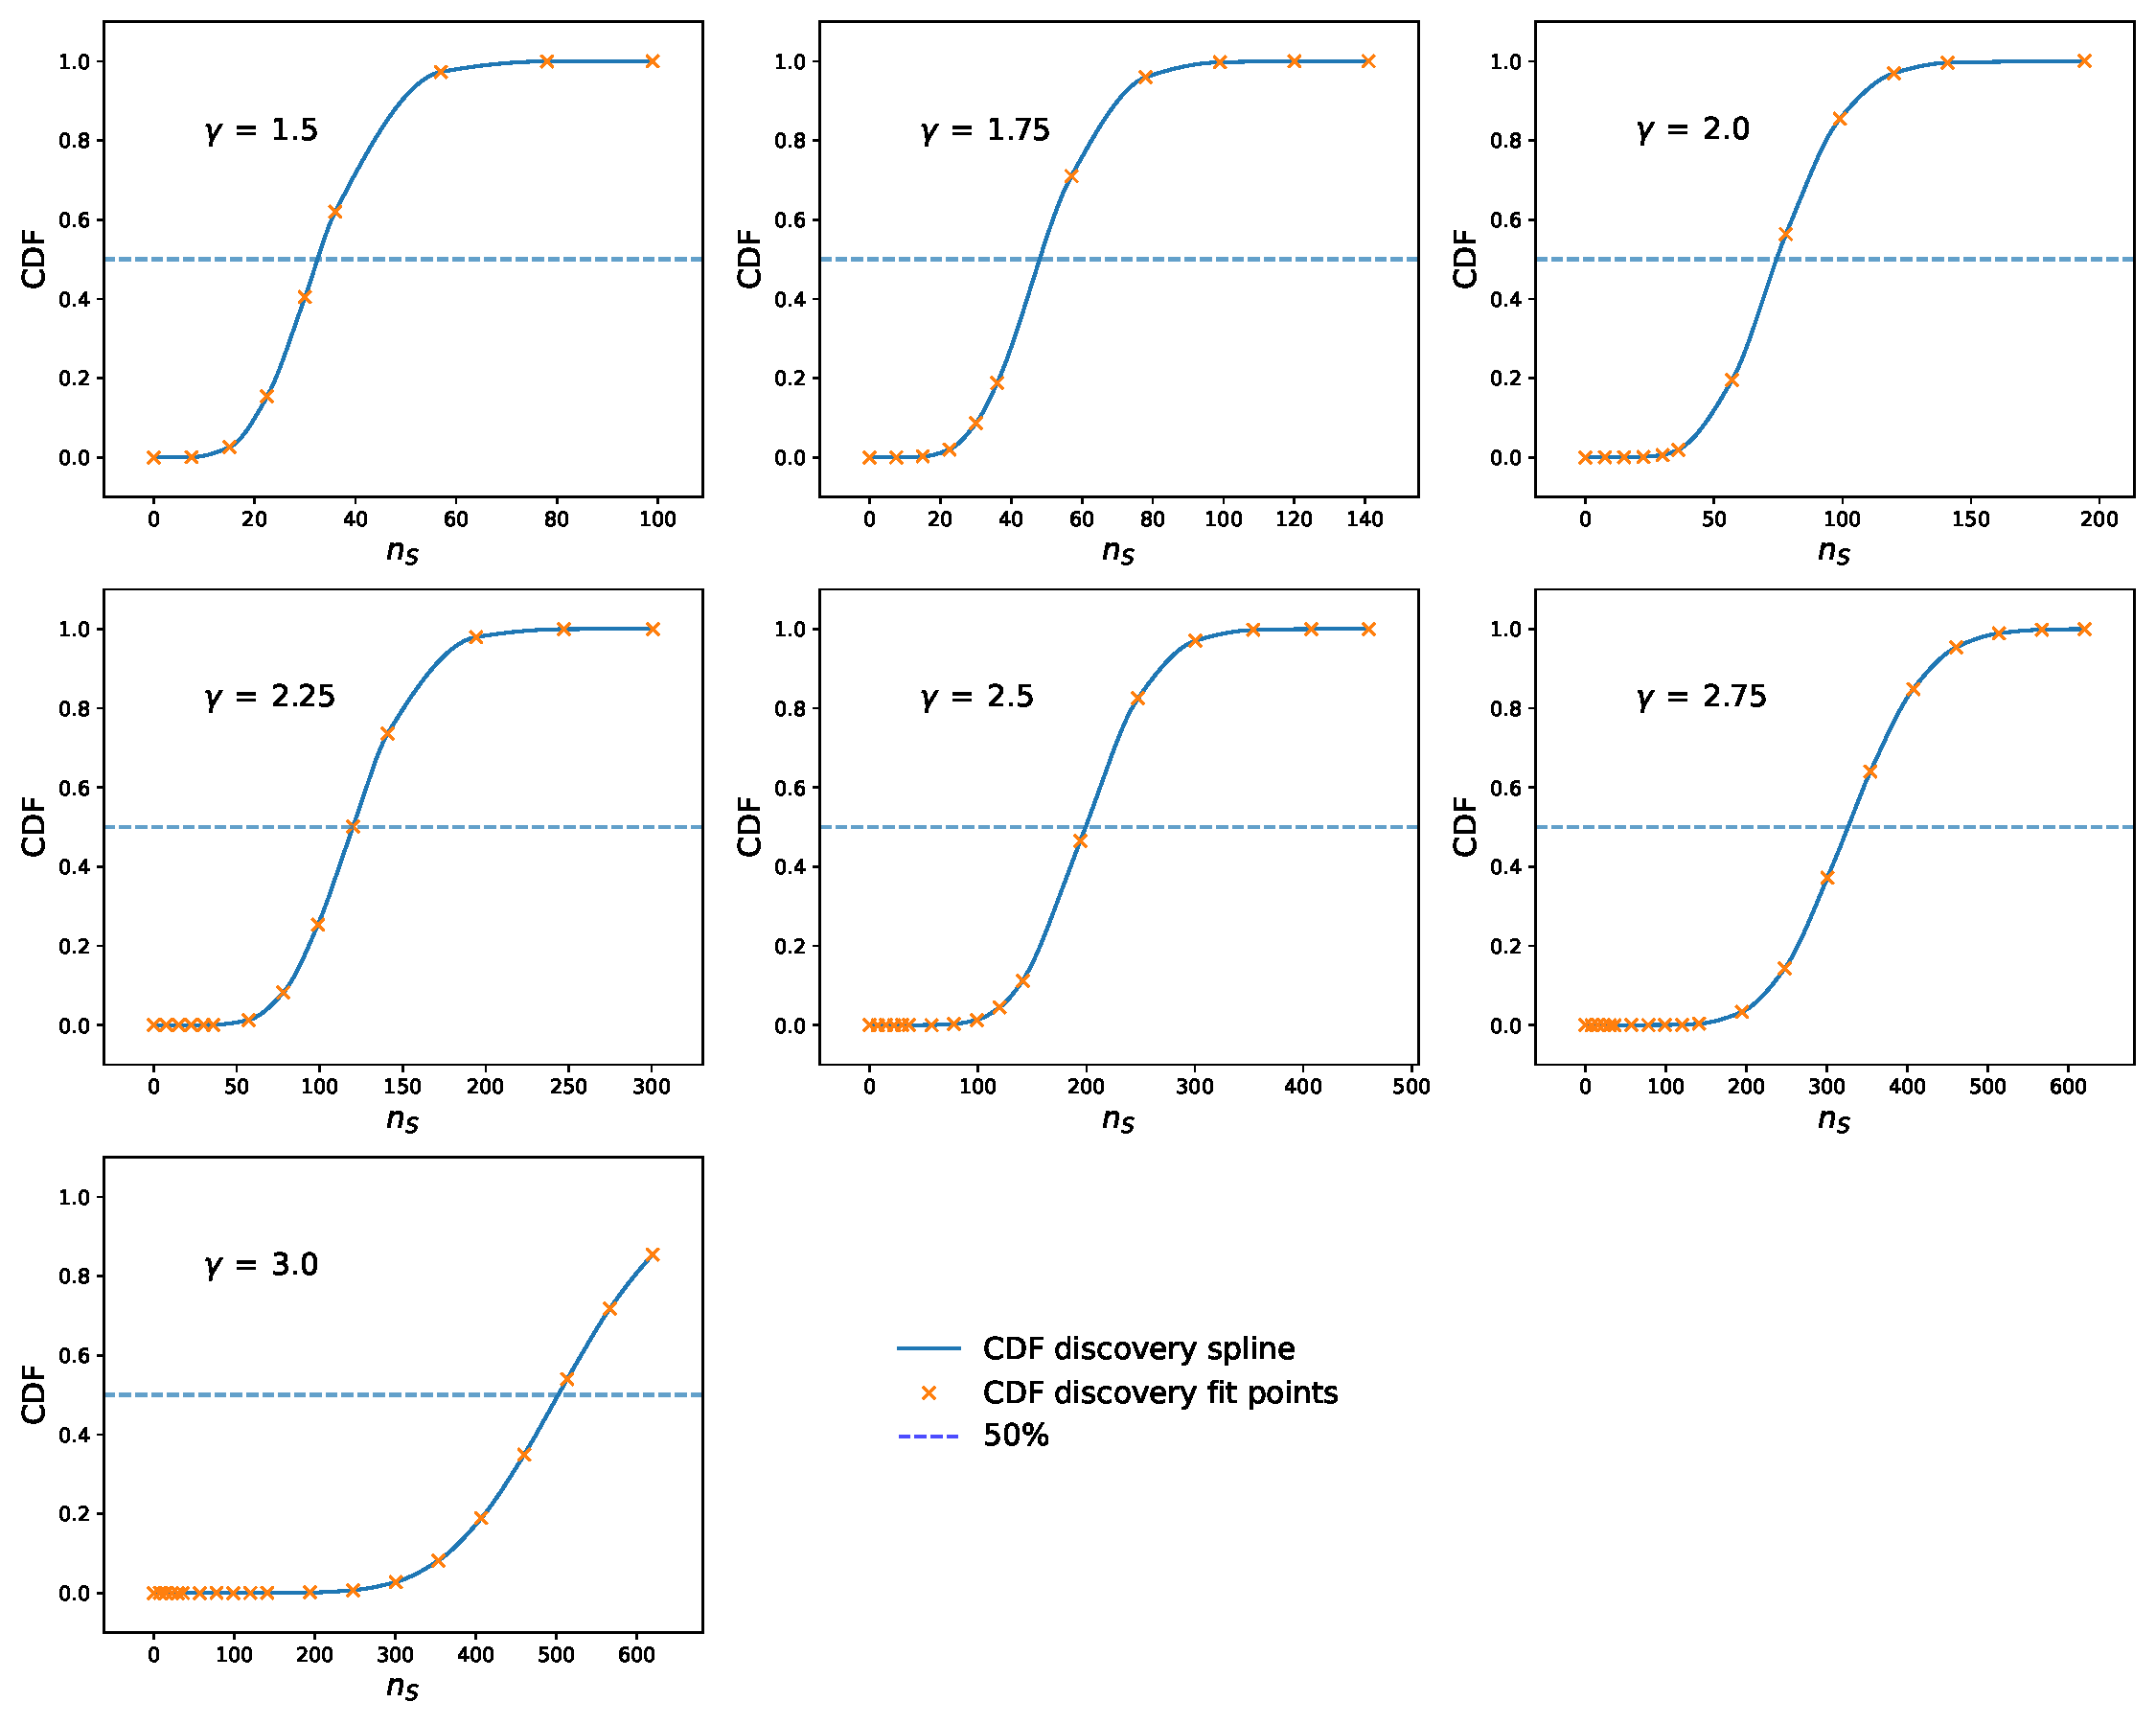
\includegraphics[width=\linewidth]{Plots/05_csky/9_years_gfu_gold_cdf_disc.pdf}
    \caption{Quantiles of the signal trials for the calculation of the discovery potential for different spectral indices $\gamma$. A $\chi^2$ CDF fit provides a more accurate estimate of the sought signal parameter $n_\text{S}$ which satisfies the condition of the discovery potential at $\SI{50}{\percent}$.}
    \label{fig:cdf_disc}
\end{figure}
The sensitivities and discovery potentials from the CDFs can be seen in figure \ref{sens_disc_time_int} and additionally in table \ref{tab:sens_disc_time_int}.
The values rise for higher spectral indices since the signal looks more background like the closer the spectral index is to $\gamma = 3$.
\begin{figure}
    \centering
    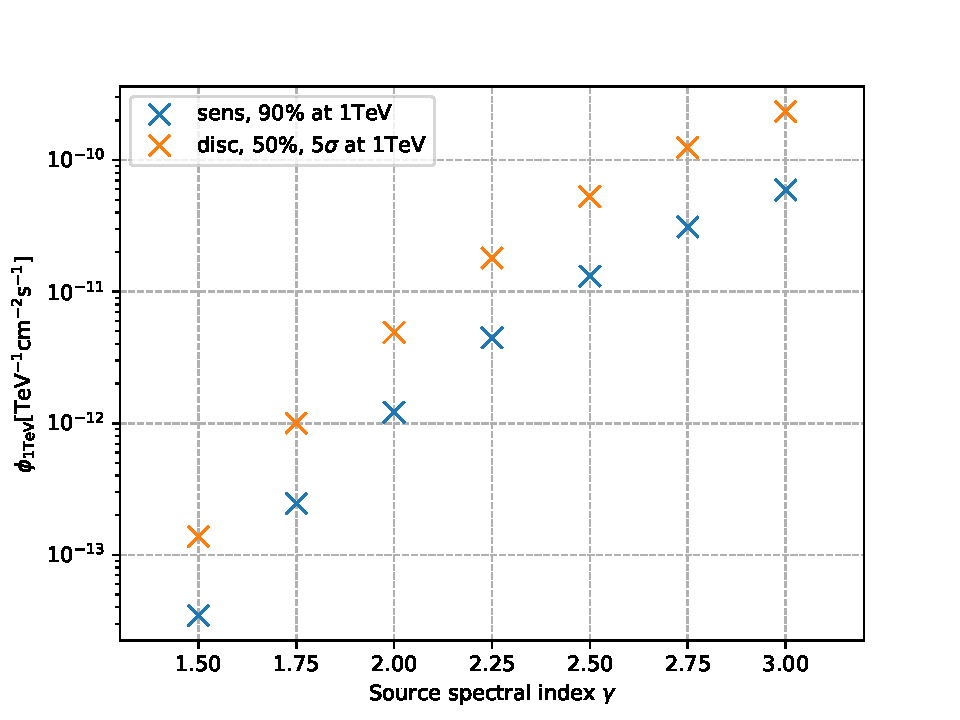
\includegraphics[width=\linewidth]{Plots/05_csky/time_int_sens_gfu_gold_9_years_new.pdf}
    \caption{Sensitivities and discovery potentials for different spectral indices $\gamma$. The reference energy is $E_0 = \SI{1}{\tera\electronvolt}$.}
    \label{fig:sens_disc_time_int}
\end{figure}


\chapter{Time-Dependent Search}

\section{Background Trials}

\begin{figure}
    \centering
    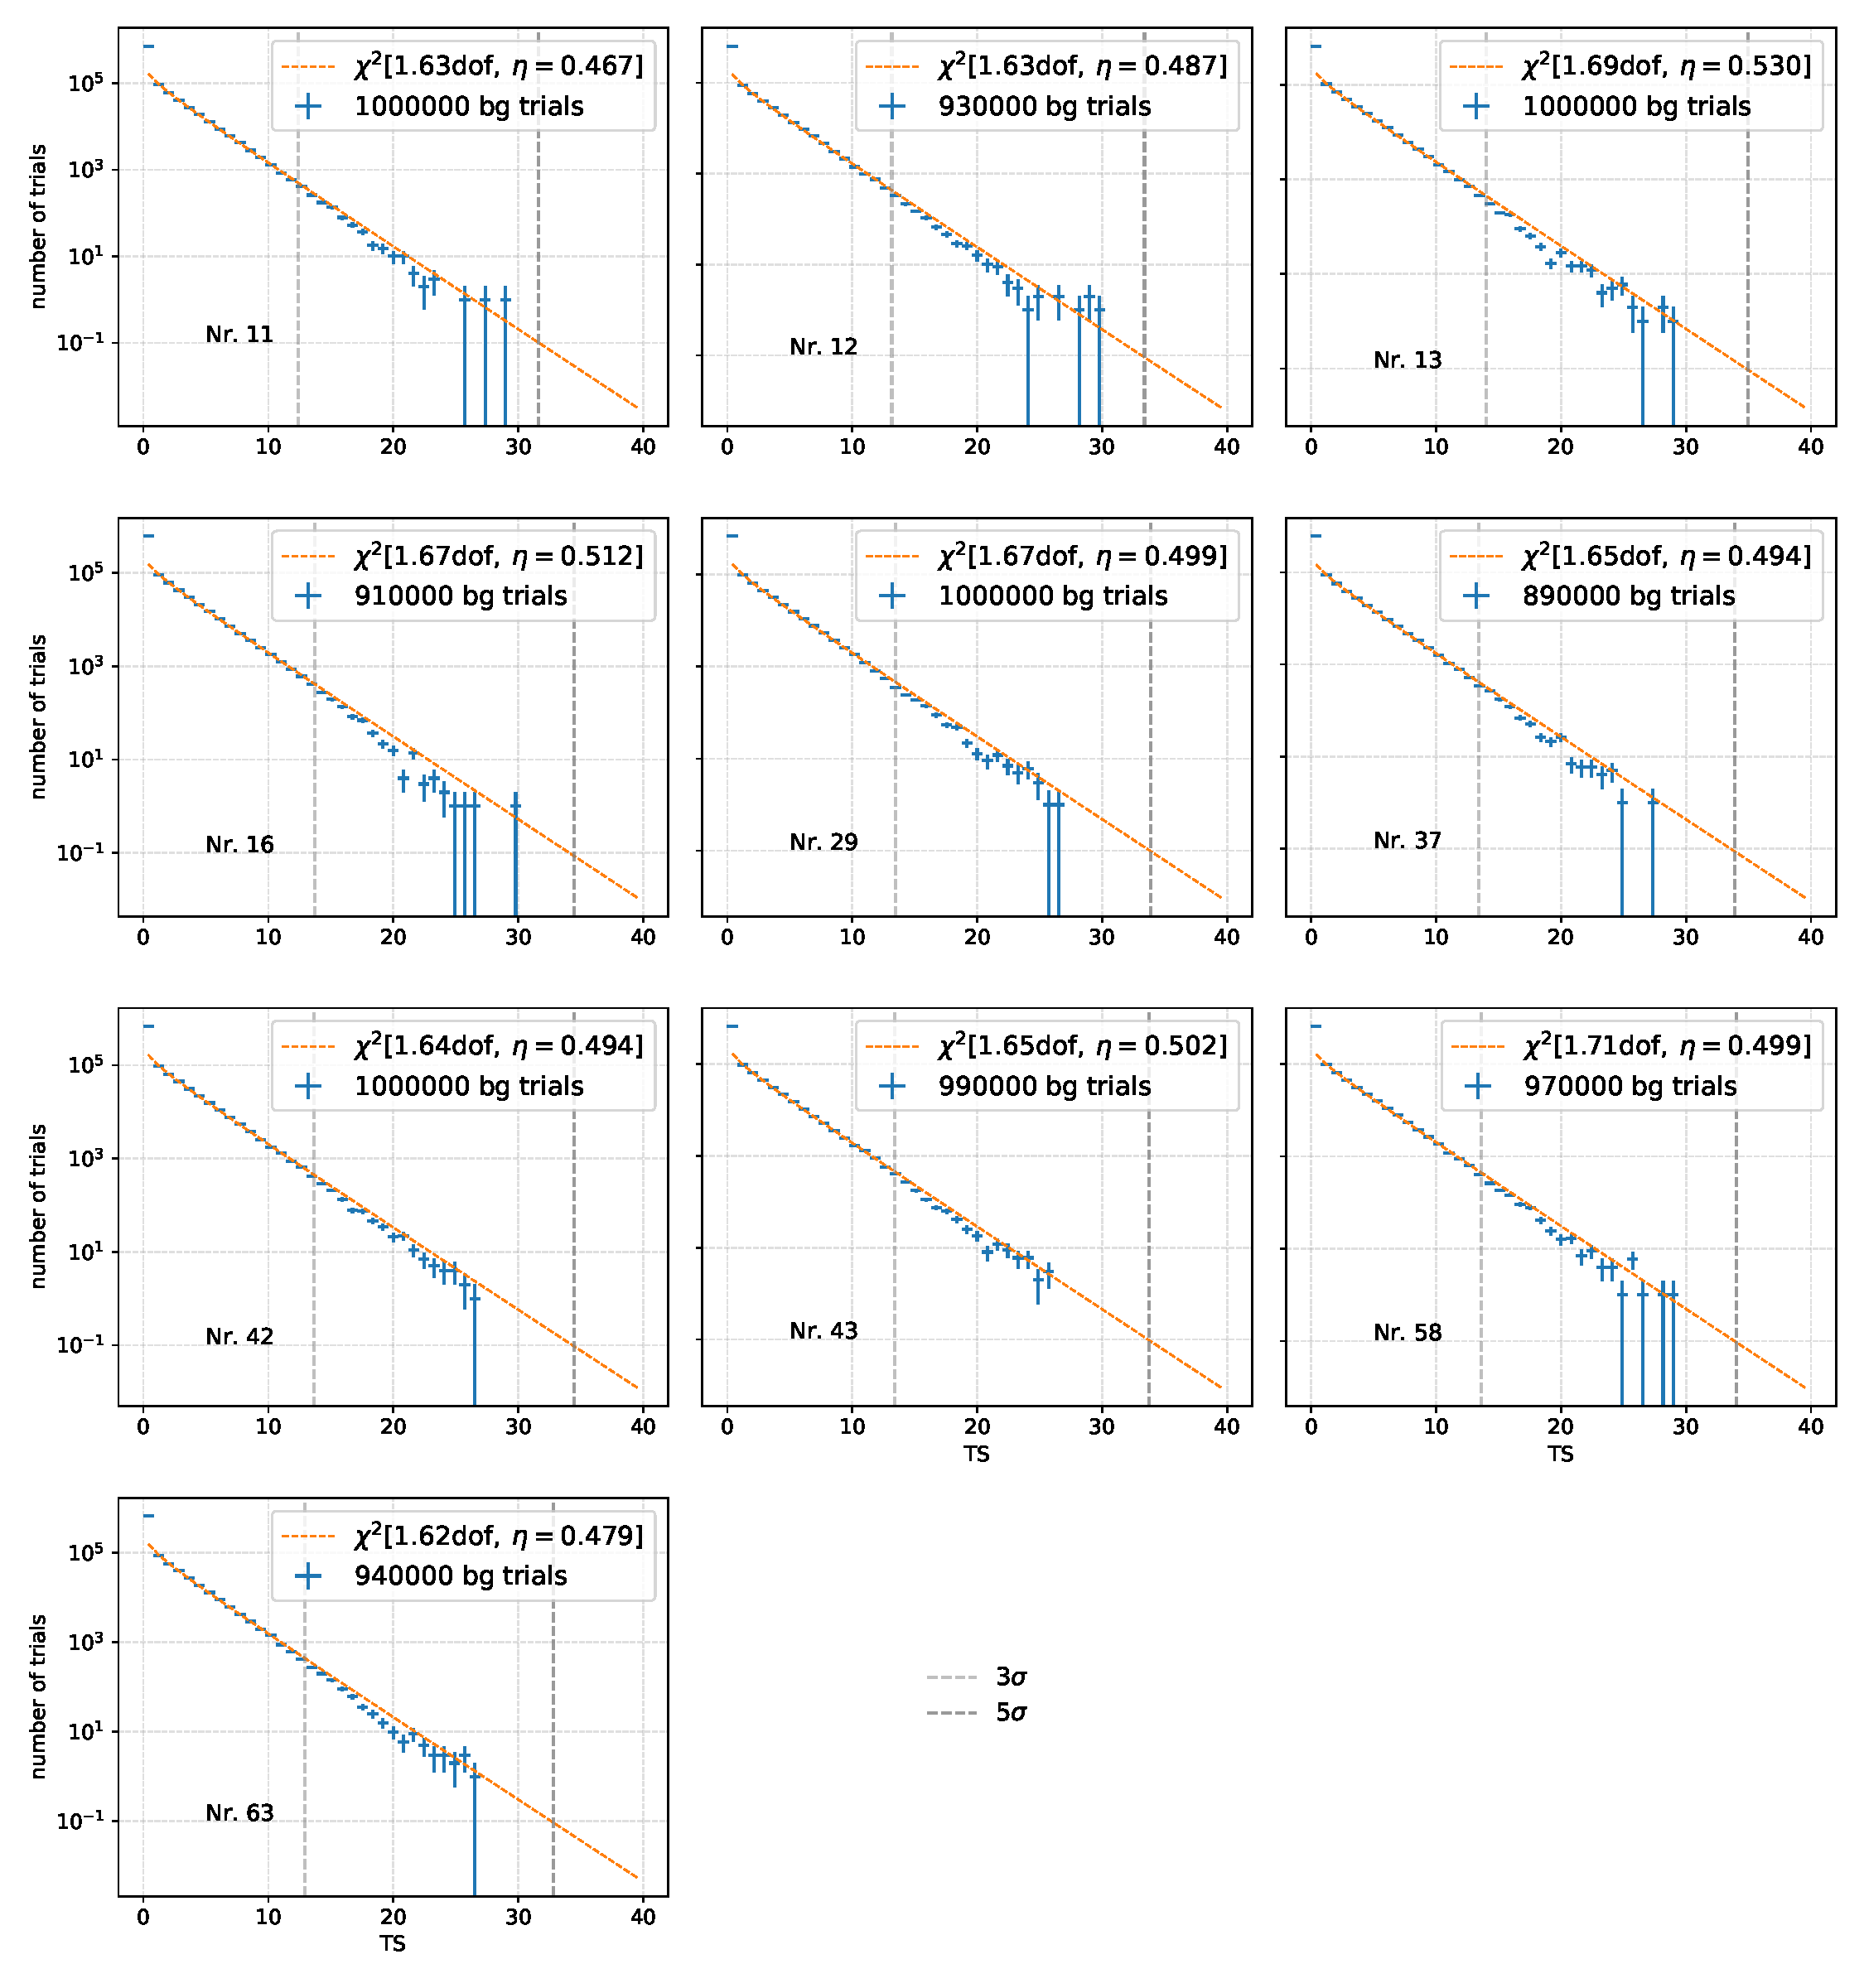
\includegraphics[width=5cm]{Plots/05_csky/9_years_gfu_gold_time_dep_bg_t0.pdf}
    \caption{.}
\end{figure}

\begin{figure}
    \centering
    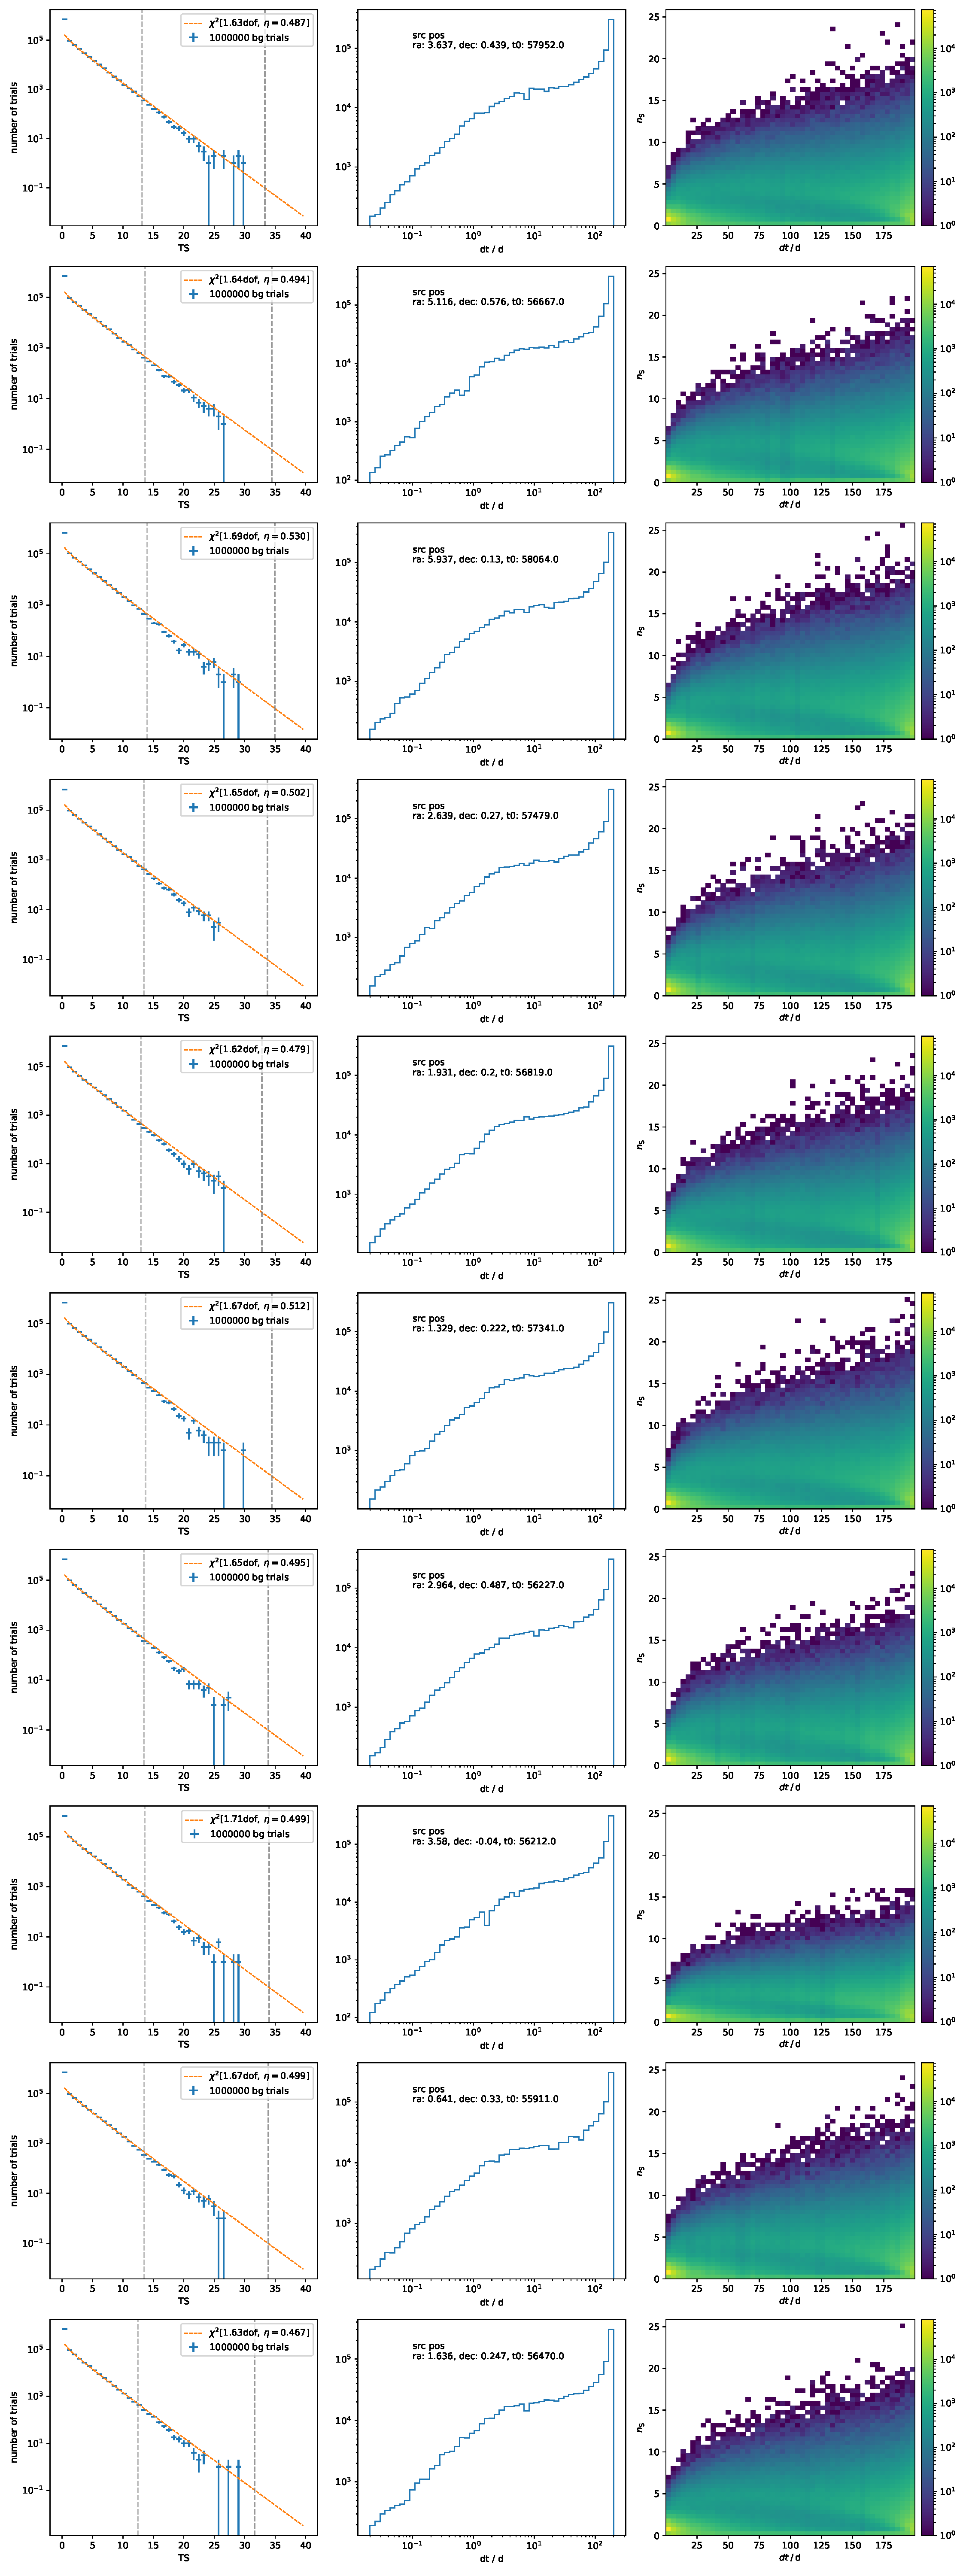
\includegraphics[width=5cm]{Plots/05_csky/9_years_gfu_gold_time_dep_bg_timewindows_fixed_t0.pdf}
    \caption{.}
\end{figure}

ns = 2 because the time box is set between 2 events, thus ns = 2 and maybe lower because of weighting (events may not look as signal like)
\section{Signal Trials}

\begin{figure}
    \centering
    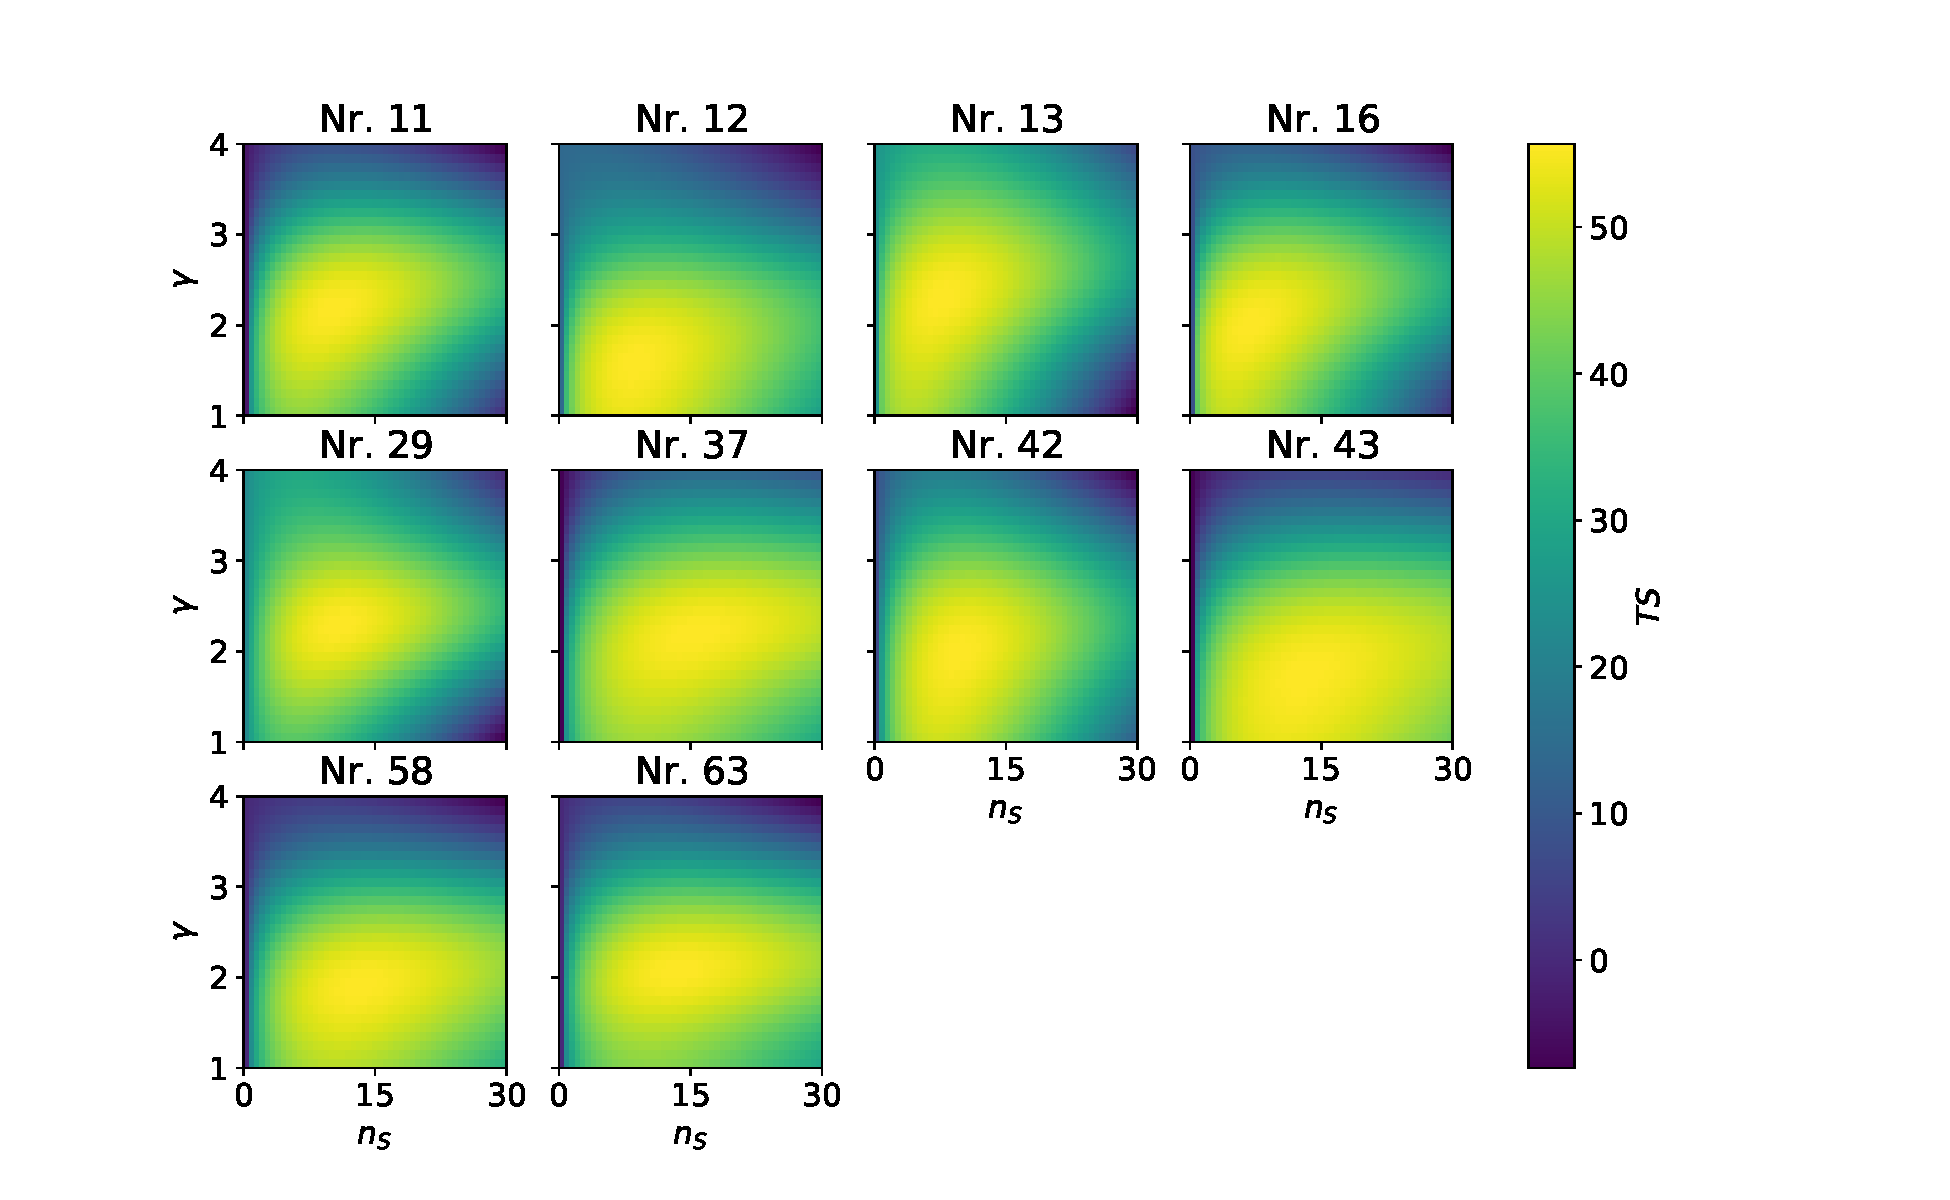
\includegraphics[width=\linewidth]{Plots/05_csky/llh_scan.pdf}
    \caption{Scan of the likelihoodspace for every source with a timewindow of $\SI{200}{\day}$. The scan is in the spectral index $\gamma$ and the signal parameter $n_S$. The source number corresponds to table \ref{tab:sources}.}
    \label{fig:llh_scan_time_dep}
\end{figure}
